\documentclass[xcolor=table]{beamer}


\let\Tiny=\tiny

\usepackage[russian]{babel}
\usepackage{cmap}
\usepackage[utf8]{inputenc}
\usepackage{amsmath}
\usepackage{color}
\usepackage[table]{xcolor}
\usepackage{float}
\title[]{Интеллектуальный анализ данных\\(Data mining)}

% Don`t know how to make title slide properly using beamer customization :(
\author[]{ \\[0.5cm]  \Large Доклад на семинаре по \\ специальности \\[1.3cm]  Студент гр.4057/2 Виктор Смолов \\ 13 декабря}

\usetheme{Darmstadt}
\usecolortheme{crane}
\useoutertheme{infolines} 
\setbeamersize{text margin left=1cm,text margin right=.5cm} 
\setbeamertemplate{navigation symbols}{}
\setbeamertemplate{headline}{}
\setbeamertemplate{footline}[page number]{}
\setbeamertemplate{caption}[numbered]

\newtheorem{defn}{Определение}
\newtheorem{prob}{Постановка задачи}

\definecolor{myGreen}{RGB}{0,201,94}
\definecolor{cell1}{RGB}{206,161,255}
\definecolor{cell2}{RGB}{160,222,176}

%{%
%\begin{flushright}{\begin{tt}\begin{LARGE}\insertframenumber/\inserttotalframenumber\end{LARGE}\end{tt}}\end{flushright}%
%}

\date[13 декабря 2010]{}
\begin{document}

\thispagestyle{empty}

\begin{frame}
  \maketitle
\end{frame}

\setcounter{page}{1}

\begin{frame}
  \frametitle{Содержание} 
  Введение \\[0.3cm]
  \tableofcontents
  Заключение \\[0.3cm]
  Использованные источники
\end{frame}

\section*{Введение}
%\addtocontents{toc}{\contentsline{section}{123}{1}}
%\addcontentsline{toc}{section}{asd}
\subsection{Определение}

\begin{frame}
  \frametitle{Введение}
  \framesubtitle{Определение}

  \begin{center}
    \colorbox{myGreen}{\LARGE{Data mining}}  
  
  \begin{picture}(200,50)
    \thicklines
    \put(60,40){\vector(-1,-1){30}}
    \put(145,40){\vector(1,-1){30}}
  \end{picture}
  
  \begin{columns}
    \begin{column}{0.5\textwidth}
       Data - данные, информация
    \end{column}
    \begin{column}{0.5\textwidth}
       Mining - добыча полезных ископаемых
    \end{column}
  \end{columns}
  \end{center}

  \begin{defn}
    Data Mining - это процесс выделения из данных неявной и неструктурированной информации и представления ее в виде, пригодном для использования.
  \end{defn}

\end{frame}

\begin{frame}
  \frametitle{Введение}
  \framesubtitle{Определение (2)}
  \begin{defn}[Григорий Пиатецкий-Шапиро, 1989]
    Data Mining - это процесс обнаружения в сырых данных ранее неизвестных, нетривиальных, практически полезных и доступных интерпретации знаний, необходимых для принятия решений в различных сферах человеческой деятельности.
  \end{defn}
  \vspace{-15pt}
  \begin{figure}
    {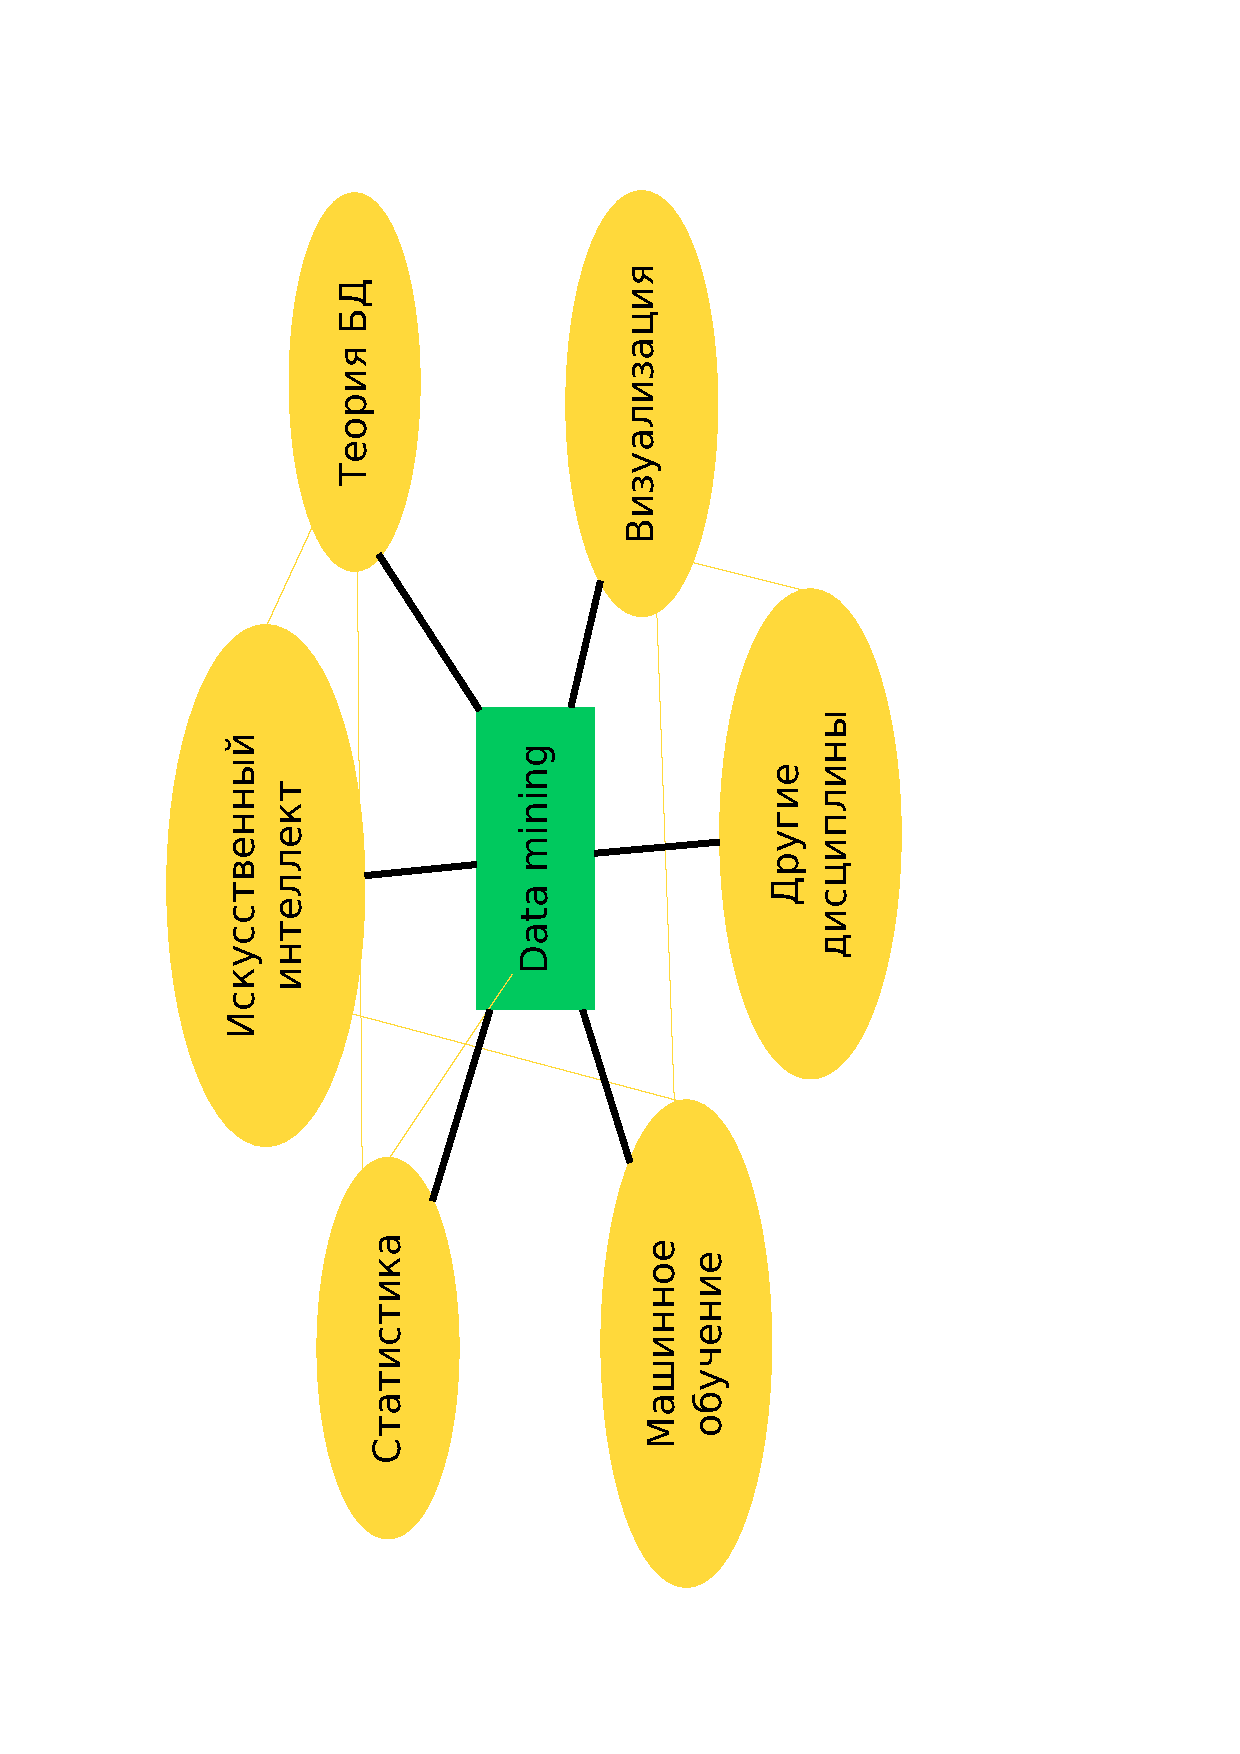
\includegraphics[angle=270,scale=0.3,clip=true,trim=23mm 25mm 53mm 30mm]{data/diag1}}
    \vspace{-5pt}
    \caption{ИАД как мультидисциплинарная наука}
  \end{figure}
\end{frame}

\begin{frame}
  \frametitle{Введение}
  \framesubtitle{Отличия от других методов анализа данных}
  В основу современной технологии Data Mining положена концепция шаблонов (паттернов), отражающих фрагменты многоаспектных взаимоотношений в данных.

  \vspace{-15pt}

  \begin{table}
    \caption{Примеры формулировок задач}
    \vspace{-10pt}
    \begin{tabular}{|p{0.5\textwidth}|p{0.45\textwidth}|}
      \hline
      \cellcolor{cell1} OLAP (online analytical processing) & \cellcolor{cell2} Data Mining \\ \hline
      \cellcolor{cell1} Каковы средние показатели травматизма для курящих и некурящих? & \cellcolor{cell2} Встречаются ли точные
      шаблоны в описаниях людей, подверженных повышенному травматизму? \\ \hline
      \cellcolor{cell1} Каковы средние размеры телефонных счетов существующих клиентов в сравнении со счетами бывших клиентов (отказавшихся от услуг телефонной компании)? &
      \cellcolor{cell2} Имеются ли характерные портреты клиентов, которые, по всей вероятности, собираются отказаться от услуг телефонной компании? \\
      \hline
    \end{tabular}
  \end{table}
\end{frame}

\subsection{Данные}

\begin{frame}
  \frametitle{Введение}
  \framesubtitle{Данные}
  
  \begin{defn}
    Данные - это необработанный материал, предоставляемый поставщиками \emph{данных} и используемый потребителями для формирования информации.
  \end{defn}

  Наиболее часто встречающиеся (обрабатываемые) данные \footnotemark:
  \begin{enumerate}
    \item Табличные данные
    \item Временные ряды
    \item Текст
    \item Графические данные: изображения, графы, карты, молекулы, web-данные
    \item Аудио/Видео
  \end{enumerate}

  \footnotetext[1]{По данным сайта \url{http://www.kdnuggets.com/}} 
\end{frame}

\begin{frame}
  \frametitle{Введение}
  \framesubtitle{Данные (2)}
  
  \begin{itemize}
  \item Для выполнения основной цели (нахождения шаблонов) нужны большие объемы информации.
    
  \item Для обработки сырых данных потребуется большое количество времени.
      
  \item Основной этап решения задачи методами ИАД - \alert{предобработка данных}.
  \end{itemize}
  
  \begin{defn}
    Предобработка данных - выделение особых, уникальных признаков из каждого наблюдения из сырых данных для уменьшения объема обрабатываемой информации и улучшения полученных результатов.
  \end{defn}

\end{frame}


\section{Задачи и методы решения}
%\contentsline {section}{Задачи и методы решения \\}
%\addtocontents{toc}{ \newline}

\subsection{Основы анализа данных}
\begin{frame}
  \frametitle{Основы анализа данных}
  \framesubtitle{Статистики}
  \vspace{-20pt}

  \begin{columns}

    \begin{column}{0.35\textwidth}
      \begin{table}
        \caption{Набор данных A}
        \begin{tabular}{|c|c|}
          \hline
          x & y \\ \hline
          3 & 9 \\ \hline 2 & 7 \\ \hline 4 & 12 \\ \hline 5 & 15 \\ \hline 6 & 17 \\ \hline
          7 & 19 \\ \hline 8 & 21 \\ \hline 9 & 23.4 \\ \hline 10 & 25.6 \\ \hline 11 & 27.8 \\
          \hline
        \end{tabular}
      \end{table}
    \end{column}

    \begin{column}{0.7\textwidth}
      \begin{table}
        \caption{Описательные статистики для набора A}
        \begin{tabular}{|c|c|c|}
          \hline
          Описательная статистика & x & y \\ \hline
          Среднее & 6,5 & 17,68 \\ \hline
          Стандартная ошибка & 0,95 & 2,21 \\ \hline
          Медиана & 6,5 & 18 \\ \hline
          Стандартное отклонение & 3,02 & 6,99 \\ \hline
          Дисперсия выборки & 9,16 & 48,88 \\ \hline
          Эксцесс & -1,2 & -1,10 \\ \hline
          Асимметричность & 0 & -0,12 \\ \hline
          Интервал & 9 & 20,8 \\ \hline
          Минимум & 2 & 7 \\ \hline
          Максимум & 11 & 27,8 \\ \hline
          Сумма & 65 & 176,8 \\ \hline
          Счет & 10 & 10 \\ \hline
          Уровень надежности (95,0\%) & 2,16 & 5,00 \\
          \hline
        \end{tabular}
      \end{table}
    \end{column}
  \end{columns}
\end{frame}

% \begin{frame}
%   \frametitle{Основы анализа данных}
%   \framesubtitle{Коэффициент корреляции}
  
% \end{frame}


\subsection{Машинное обучение}
\begin{frame}
  \frametitle{Машинное обучение}
  \begin{defn}
    Машинное обучение (англ. Machine Learning) — обширный подраздел искусственного интеллекта, изучающий методы построения алгоритмов, способных обучаться.
  \end{defn}

  \vspace{25pt}

  Задачи машинного обучения разделяются на:
  \begin{itemize}
  \item Обучение с учителем    
  \item Обучение без учителя
  \end{itemize}
\end{frame}

% \begin{frame}
%   \frametitle{Машинное обучение}
%   \framesubtitle{Обучение с учителем}
% \end{frame}

% \begin{frame}
%   \frametitle{Машинное обучение}
%   \framesubtitle{Обучение без учителя}
% \end{frame}


\subsection{Классификация}
\begin{frame}
  \frametitle{Классификация}
  \framesubtitle{Постановка задачи}
  
  \begin{prob}
    Пусть $X$ - множество описаний объектов, $Y$ - конечное множество номеров (имен, меток) классов.
    Существует неизвестная \emph{целевая зависимость} -- отображение $y^*: X \rightarrow Y$, значения которой
    известны только на объектах конечной обучающей выборки $S = \{(x_1, y_1), \dots, (x_m, y_m)\}$.
    Требуется построить алгоритм $A: X \rightarrow Y$, способный классифицировать произвольный объект $x \in X$.
  \end{prob}

  \vspace{-15pt}

  \begin{center}
    \begin{figure}
      \caption{Пример. Классификация зеленого треугольника}
      \vspace{-5pt}
      \fbox{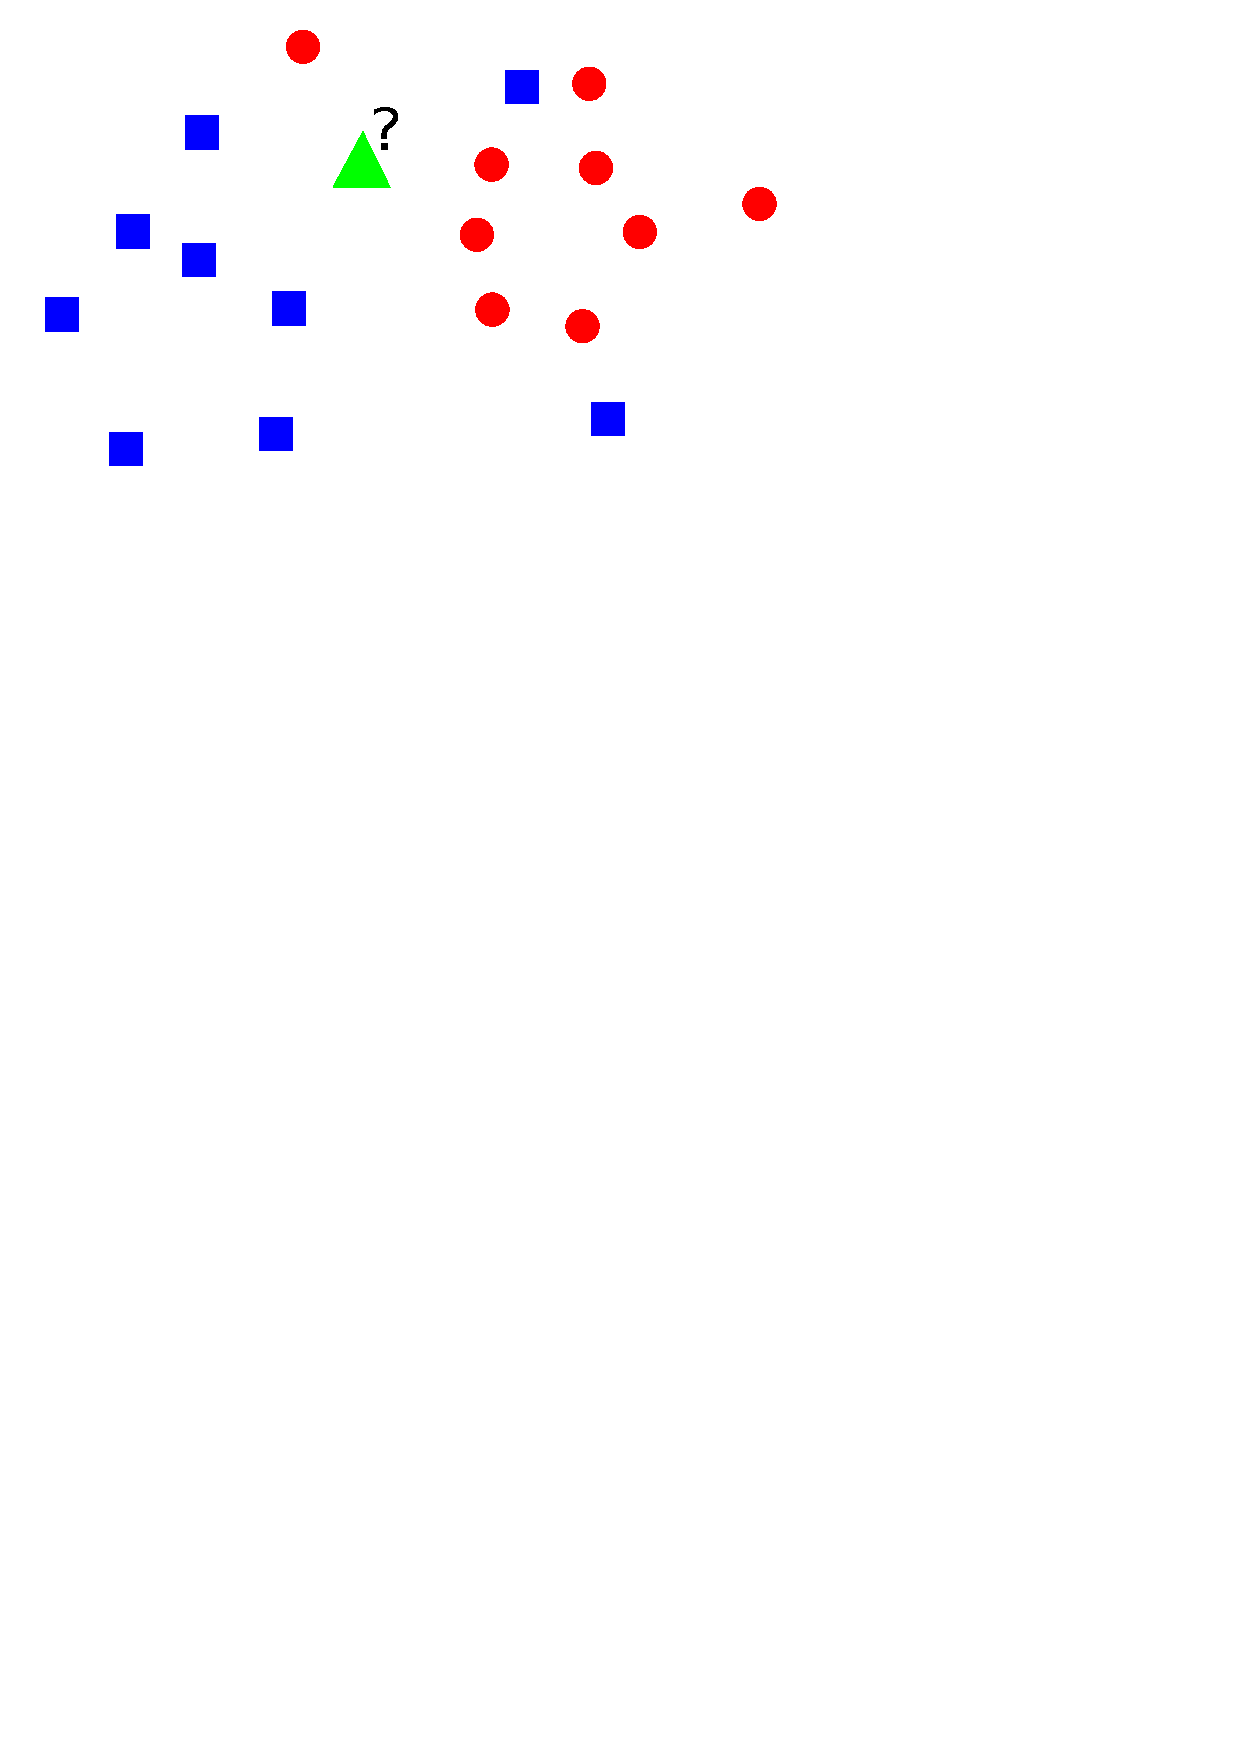
\includegraphics[scale=0.4,clip=true,trim=5mm 215mm 75mm 5mm]{data/class}}
    \end{figure}
  \end{center}
\end{frame}

\begin{frame}
  \frametitle{Классификация}
  \framesubtitle{k ближайших соседей (k-NN)}

  \begin{columns}
    \begin{column}{0.4\textwidth}
      \fbox{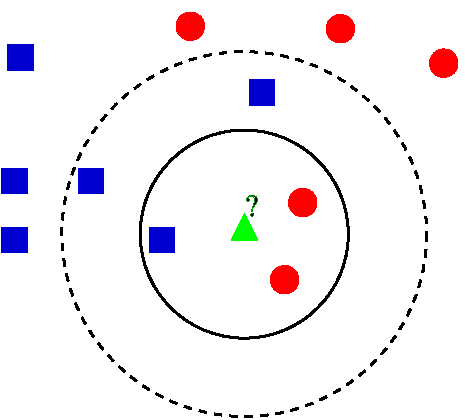
\includegraphics[scale=0.55]{data/knn}}
    \end{column}
    \begin{column}{0.6\textwidth}
      Для произвольного объекта $x$ расположим объекты обучающей выборки в порядке возрастания расстояния до $x$:
      \[\rho(x, x_{1;x}) < \dots < \rho(x, x_{m;x})\]

      Обобщеная формула классификации:
      \vspace{-10pt}
      \[A(x) = \operatorname*{arg\,max}_{y \in Y}{\sum_{i=1}^m[x_{i;x} = y] \cdot w(i, x)}\]
    \end{column}
  \end{columns}  

  $w(i, x)$ - весовая функция:
  \begin{itemize}
  \item $w(i, x) = [i = 1]$ - метод ближайшего соседа
  \item $w(i, x) = [i \leq k]$ - метод k ближайших соседей
  \item $w(i, x) = [i \leq k] \cdot q^i,~(q < 1)$ - метод k экспоненциально взвешенных ближайших соседей
  \end{itemize}
\end{frame}

\begin{frame}
  \frametitle{Классификация}
  \framesubtitle{Практическое применение}

  \begin{columns}

  \begin{column}{0.5\textwidth}
    {\includegraphics[scale=0.35]{data/faces.png}}
  \end{column}

  \begin{column}{0.5\textwidth}
    \begin{itemize}
    \item Компьютерное зрение:
      \begin{itemize}
      \item OCR
      \item Системы слежения
      \end{itemize}
    \item Создание новых лекарств. QSAR
    \item Распознавание речи
    \item Поисковые системы
    \item Обработка естественных языков
    \end{itemize}
    \end{column}
  \end{columns}
\end{frame}


\subsection{Клаcтеризация}
\begin{frame}
  \frametitle{Кластеризация}
  \framesubtitle{Постановка задачи}

  \begin{center}
    \fbox{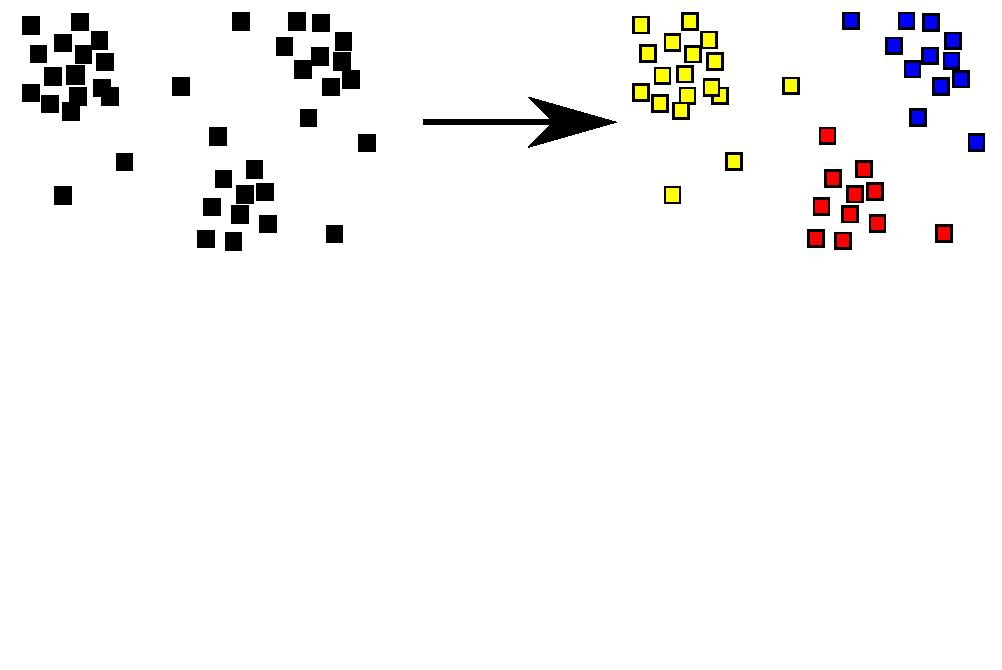
\includegraphics[scale=0.5,clip=true,trim=0mm 70mm 0mm 0mm]{data/cluster}}
  \end{center}

  \begin{prob}
    Пусть $X$ -- множество объектов, $Y$ -- множество номеров (имён, меток) кластеров. Задана функция расстояния между объектами $\rho(x, x')$.
    Имеется конечная обучающая выборка объектов $S = \{x_1, \dots, x_m\} \subset X$. Требуется разбить выборку на непересекающиеся
    подмножества, называемые \emph{кластерами}, так, чтобы каждый кластер состоял из объектов, близких по метрике $\rho$,
    а объекты разных кластеров существенно отличались. При этом каждому объекту $x_i \in S$ приписывается номер кластера $y_i$.
  \end{prob}
\end{frame}

\begin{frame}
  \frametitle{Кластеризация}
  \framesubtitle{Типы кластеризации}

  \begin{columns}
    \begin{column}{0.4\textwidth}
      Методы кластерного анализа можно разделить на две группы:
      \begin{itemize}
      \item иерархические
      \item неиерархические
      \end{itemize}
    \end{column}
    
    \begin{column}{0.6\textwidth}
      Иерархические:
      \fbox{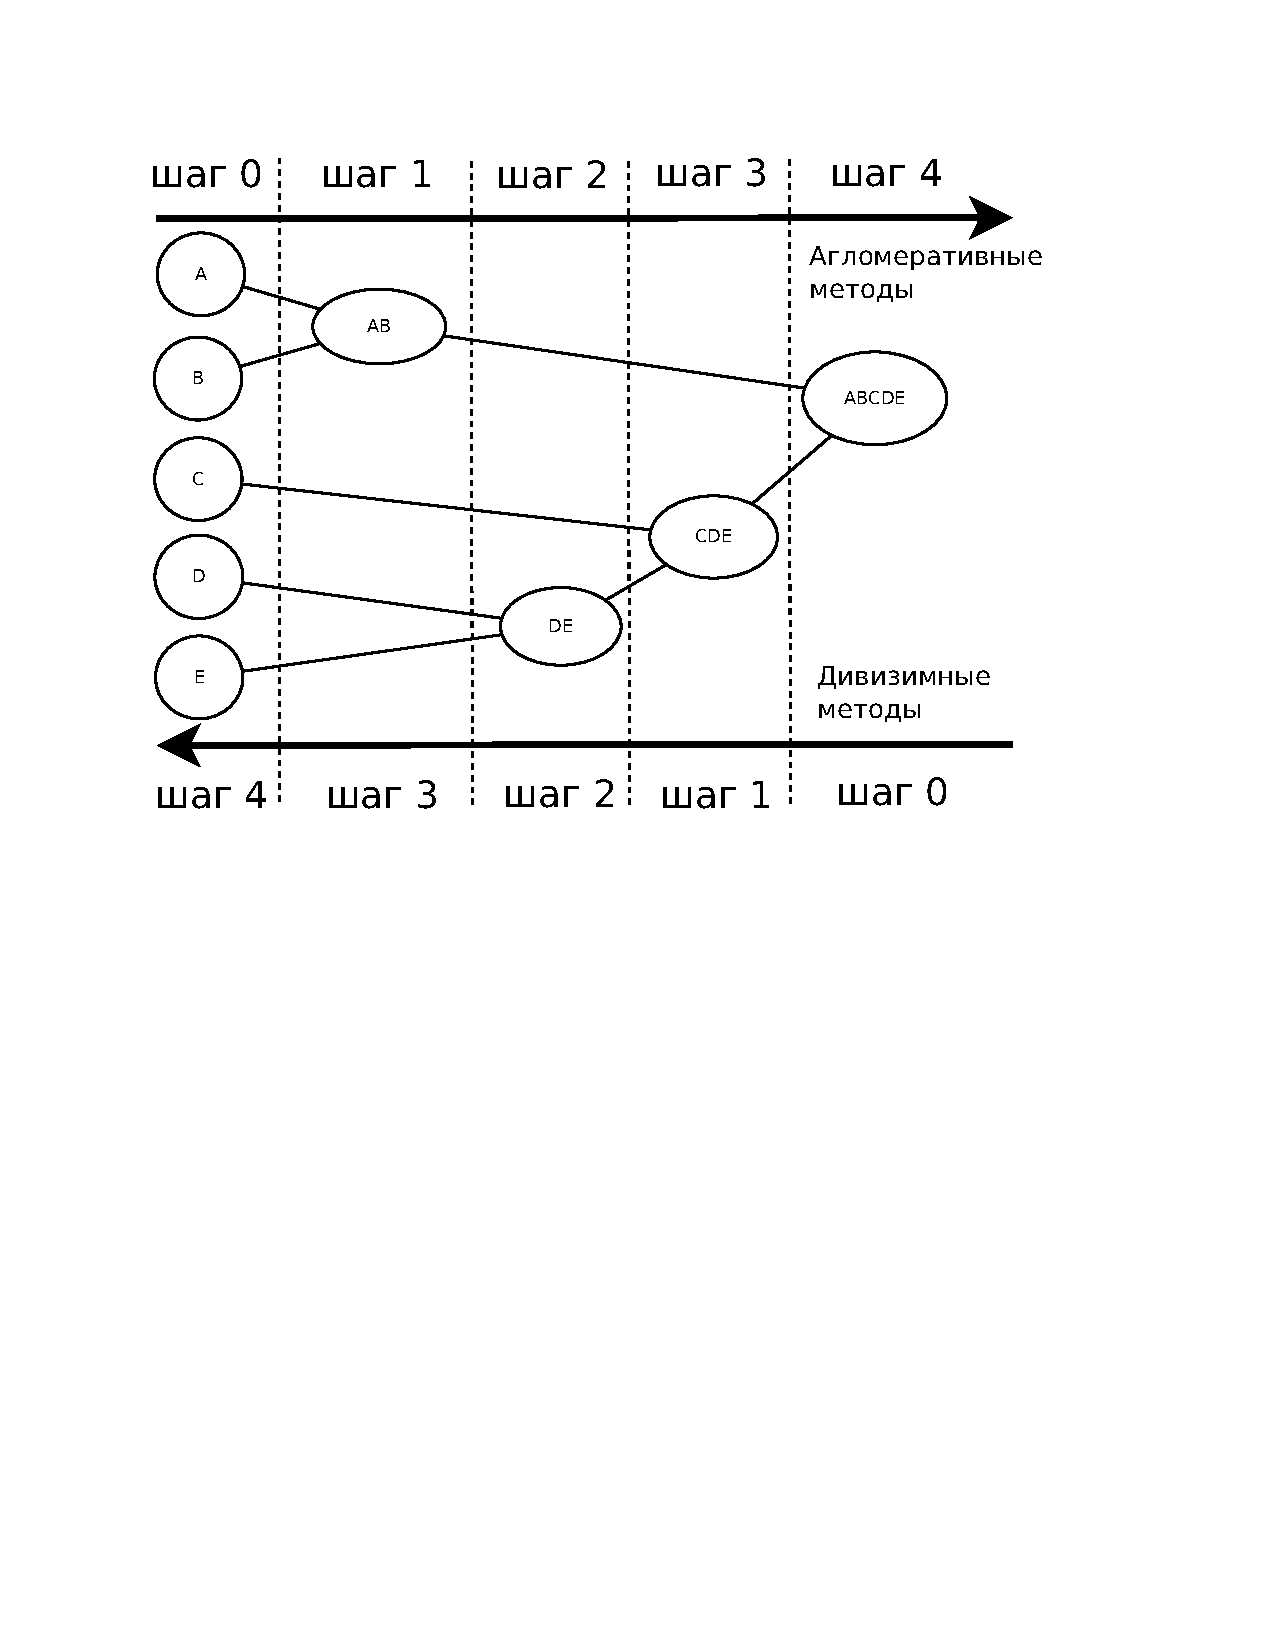
\includegraphics[scale=0.4,clip=true,trim=25mm 140mm 37mm 25mm]{data/hierarchical}}
    \end{column}
   
  \end{columns}
  \begin{defn}
    Дендрограмма (dendrogram) - древовидная диаграмма, содержащая n уровней, каждый из которых соответствует одному из шагов процесса последовательного укрупнения кластеров.
  \end{defn}
  
\end{frame}

\begin{frame}
  \frametitle{Кластеризация}
  \framesubtitle{Иерархическая кластеризация}

  \begin{center}
    Основная идея - объединение близко расположенных кластеров
  \end{center}

  \begin{columns}
    \begin{column}{0.5\textwidth}
      Исходные данные:
      \fbox{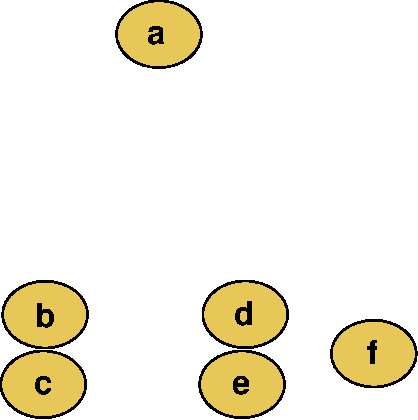
\includegraphics[scale=0.5]{data/clusters_orig}}

      Типичные функции расстояния между кластерами $A, B$:
      \begin{itemize}
      \item $\max\{d(x, y): x \in A, y \in B\}$
      \item $\min\{d(x, y): x \in A, y \in B\}$
      \item $\frac{1}{|A| \cdot |B|} \sum_{x \in A}\sum_{y \in B}d(x, y)$
      \end{itemize}
    \end{column}

    \begin{column}{0.5\textwidth}
      Дендрограмма кластеризации:
      \fbox{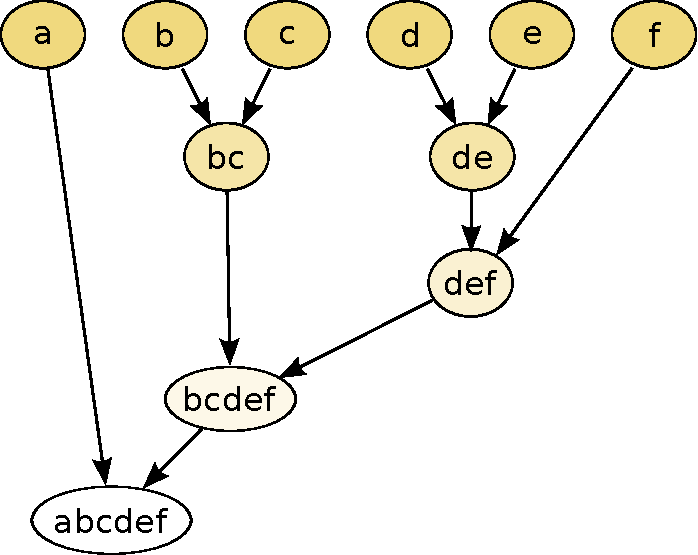
\includegraphics[scale=0.48]{data/clusters_dendr}}
    \end{column}
  \end{columns}
\end{frame}

\begin{frame}
  \frametitle{Кластеризация}
  \framesubtitle{k средних}

  \begin{columns}
    \begin{column}{0.5\textwidth}
      \begin{center}
        \fbox{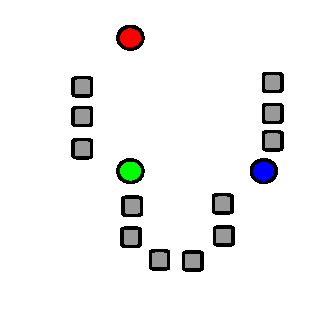
\includegraphics[scale=0.5,clip=true,trim=0mm 7.5mm 0mm 0mm]{data/km-s1}}
        \\Шаг 1. Выбор начальных центров кластеров.       
        
        \fbox{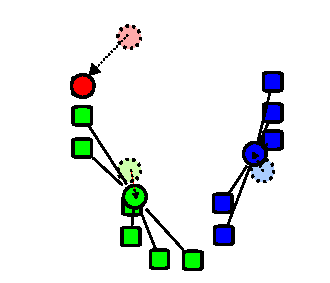
\includegraphics[scale=0.5,clip=true,trim=0mm 1.5mm 0mm 0mm]{data/km-s3}}
        \\Шаг 3. Вычисление новых центров.
      \end{center}
    \end{column}
    
    \begin{column}{0.5\textwidth}
      \begin{center}
        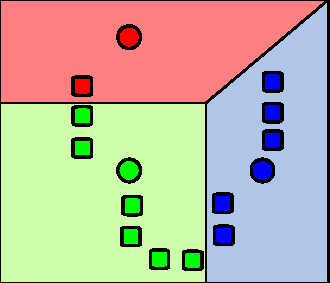
\includegraphics[scale=0.5]{data/km-s2}
        \\Шаг 2. Создание k кластеров. Диаграмма Вороного.

        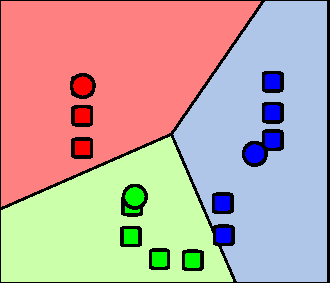
\includegraphics[scale=0.5]{data/km-s4}
        \\Шаг 4. Повторять шаги 2, 3, пока кластеры изменяются.
      \end{center}
    \end{column}
  \end{columns}
\end{frame}

\begin{frame}
  \frametitle{Кластеризация}
  \framesubtitle{Практическое применение}

  \begin{columns}
    \begin{column}{0.4\textwidth}
      \begin{figure}
        \includegraphics[scale=0.08]{data/cluster_gene}
        \caption{Кластеризация генов}
        \end{figure}
    \end{column}
    
    \begin{column}{0.6\textwidth}
      \begin{itemize}
      \item Группирование результатов поиска
      \item Сегментация изображения
      \item Может быть использован для дифференцирования различных тканей и крови на ПЭТ-снимках
      \item Нахождение сообществ в социальных сетях
      \item Разделение web-страниц по жанрам
      \end{itemize}
    \end{column}
  \end{columns}
\end{frame}

\subsection{Регрессия}

\begin{frame}
  \frametitle{Регрессия. Прогнозирование}
  \framesubtitle{Постановка задачи}

  \begin{defn}
    Регрессия — зависимость математического ожидания (например, среднего значения) случайной величины от одной или нескольких других случайных величин (свободных переменных), то есть $E(y|x) = f(x)$.
  \end{defn}
  Применяется для \alert{прогнозирования} и \alert{предсказывания}.\\
  Регрессия может быть представлена в виде суммы неслучайной и случайной составляющих.
  \[y = f(x) + \nu\]
  где $f$ — функция регрессионной зависимости, а $\nu$ — аддитивная случайная величина с нулевым матожиданием.
\end{frame}

\begin{frame}
  \frametitle{Регрессия. Прогнозирование}
  \framesubtitle{Постановка задачи (2)}

  \begin{prob}
    Задана выборка — множество $\{x_1, \dots, x_N | x \in R^M\}$ значений свободных переменных и множество $\{y_1, \dots, y_N | y \in R \}$ соответствующих 
    им значений зависимой переменной. Эти множества обозначаются как $D$, множество исходных данных $\{(x_i, y_i)_i\}$. Задана регрессионная модель (гипотеза) 
    — параметрическое семейство функций $f(w,x)$ зависящая от параметров $w \in R^W$ и свободных переменных $x$. Требуется найти наиболее вероятные параметры $\overline{w}$:
    \vspace{-10pt}
    \[
    \overline{w} = \operatorname*{arg\,max}_{w \in R^W}p(y | x, w, f) = \operatorname*{arg\,max}_{w \in R^W}p(D, w, f)
    \]
  \end{prob}
\end{frame}

\begin{frame}
  \frametitle{Регрессия. Прогнозирование}
  \framesubtitle{Линейная регрессия}

  Функция $f$ зависит от параметров  линейно. При этом линейная зависимость от свободной переменной  необязательна.
  \[ y = f(w, x) + \nu = \sum_{j=1}^N{w_j \cdot g_j(x)} + \nu\]
  Значения параметров в случае линейной регрессии находят с помощью \alert{метода наименьших квадратов}. \\
  Разности $y_i - f(x_i)$ между фактическими значениями зависимой переменной и восстановленными называются \textbf{регрессионными остатками (residuals)}.
  \[SSE~(\text{Sum of Squared Errors}) = |f(x) - y|_2 = \sum_{j=1}^N(y_i - f(x_i))^2\]
  \[MSE~(\text{Mean Square Error}) = \frac{SSE}{N - 2}\]
\end{frame}

\begin{frame}
  \frametitle{Регрессия. Прогнозирование}
  \framesubtitle{Пример}

  \begin{columns}
    \begin{column}{0.5\textwidth}
      {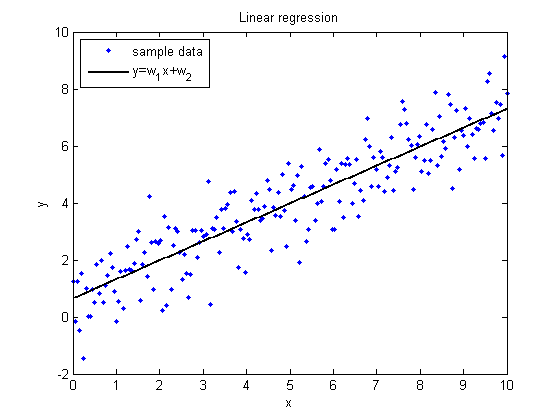
\includegraphics[scale=0.33]{data/regr1.png}}
    \end{column}

    \begin{column}{0.5\textwidth}
      {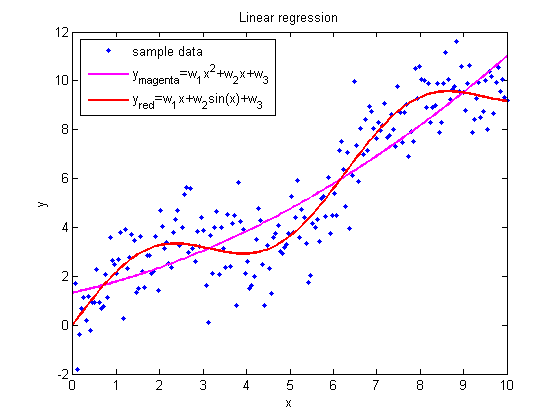
\includegraphics[scale=0.33]{data/regr2.png}}
    \end{column}
  \end{columns}
\end{frame}

\section*{Заключение}
\begin{frame}
  \frametitle{Заключение}

  \begin{itemize}
    \item Рынок систем Data Mining экспоненциально развивается
    \item Системы Data Mining применяются по двум основным направлениям:
      \begin{itemize}
        \item как массовый продукт для бизнес-приложений
        \item как инструменты для проведения уникальных исследований (генетика, химия, медицина и пр.)
      \end{itemize}
    \item Data mining - не панацея. Всё зависит от подготовки и качества данных
  \end{itemize}
\end{frame}

\begin{frame}
  \frametitle{Список литературы}

  \begin{enumerate}
    \item Википедия (англ., рус.)
    \item \url{http://www.machinelearning.ru}
    \item \url{http://www.intuit.ru/department/database/datamining}
    \item \url{http://www.inftech.webservis.ru/it/database/datamining/ar2.html}
  \end{enumerate}
\end{frame}


\begin{frame}
  \frametitle{}
  \framesubtitle{}

  \begin{center}\LARGE{Спасибо за внимание!}\end{center}
\end{frame}

\end{document}